\begin{frame}
    \frametitle{More limitations and future work}
    \begin{itemize}
    \item Ignores other externalities, like nonproliferation
        safeguards
    \begin{itemize}
        \item Incorporate potential safeguards measures into models
        \item Account for construction time and/or licensing
    \end{itemize}
    \item Expand analysis on impurities in \gls{HALEU}
    \begin{itemize}
        \item Consider power-peaking factors
        \item Model burnable poisons and control rods 
        \item Model core in non-isothermal state
    \end{itemize}
\end{itemize}
\end{frame}

\begin{frame}
    \frametitle{Once-through feed uranium}
    \begin{figure}
        \centering 
        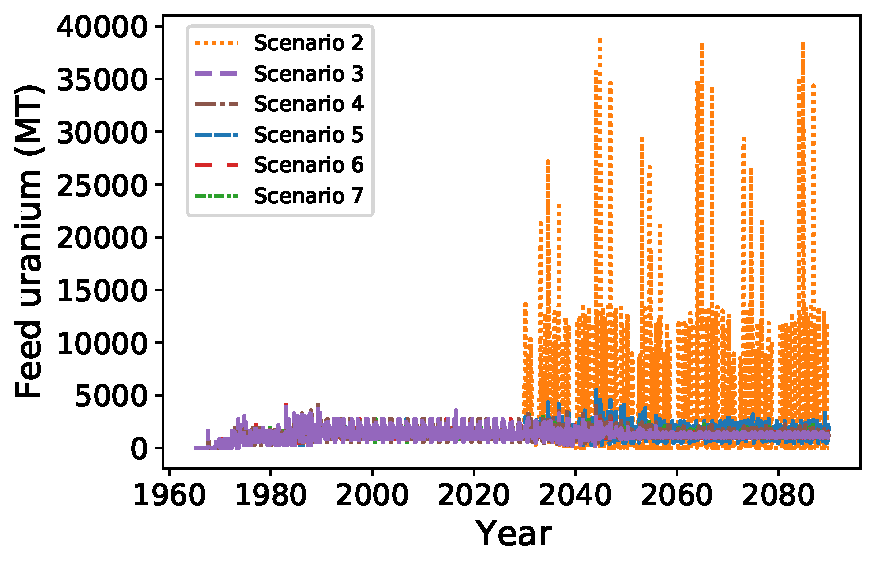
\includegraphics[scale=0.5]{nogrowth_feed.pdf}
    \end{figure}
\end{frame}

\begin{frame}
    \frametitle{Recycle HLW}
    \begin{figure}
        \centering
        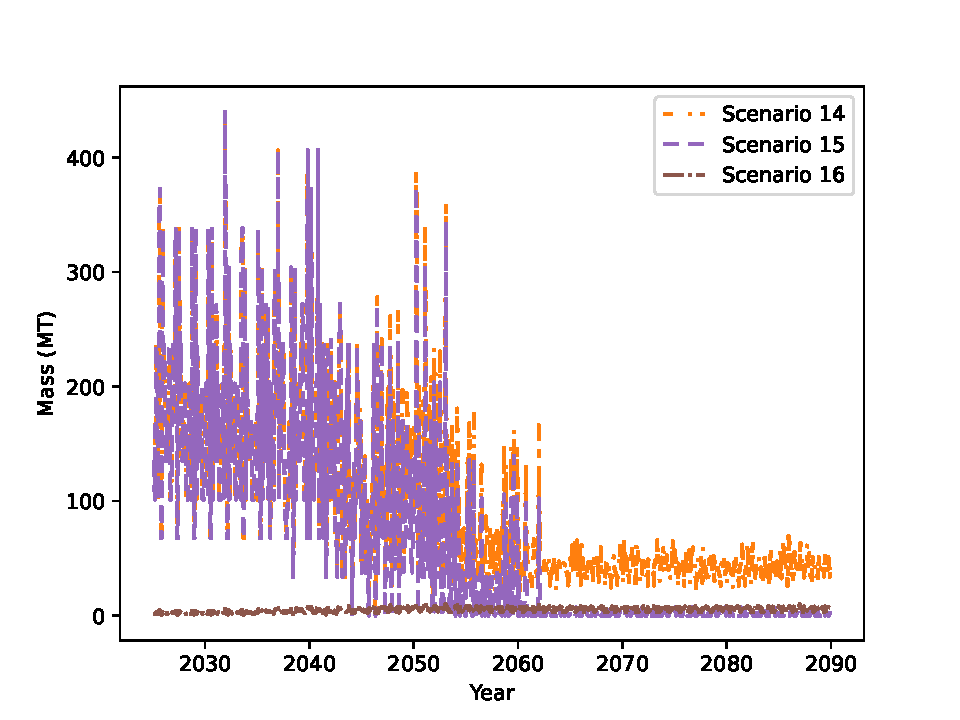
\includegraphics[scale=0.5]{nogrowth_recycle_hlw.pdf}
    \end{figure}
\end{frame}

\begin{frame}
    \frametitle{Recycle SNF}
    \begin{figure}
        \centering
        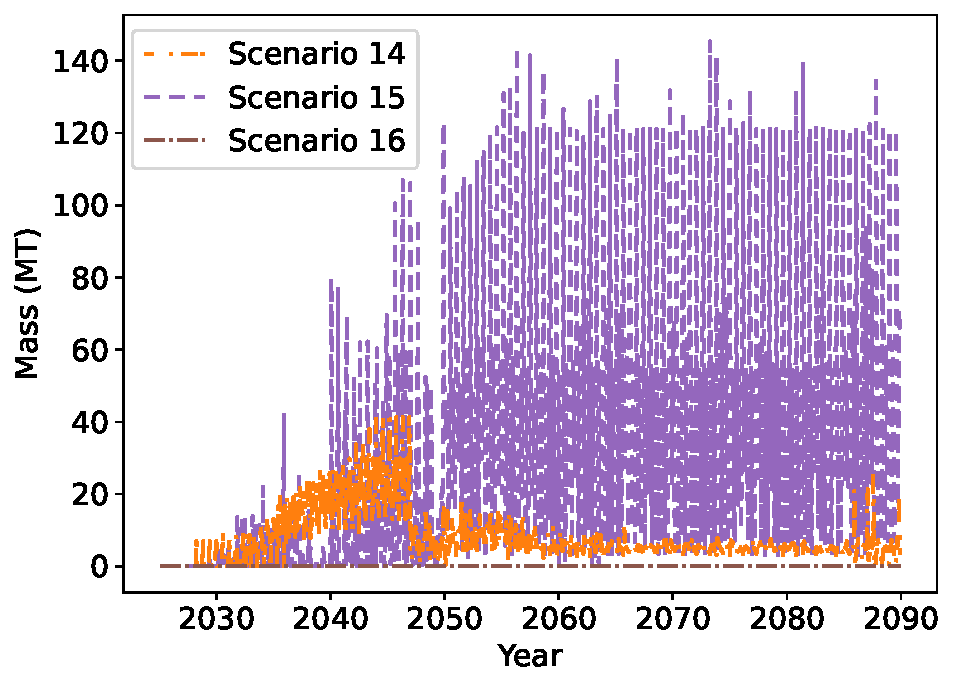
\includegraphics[scale=0.5]{nogrowth_recycle_snf.pdf}
    \end{figure}
\end{frame}

\begin{frame}
    \frametitle{Recycle SWU}
    \begin{figure}
        \centering
        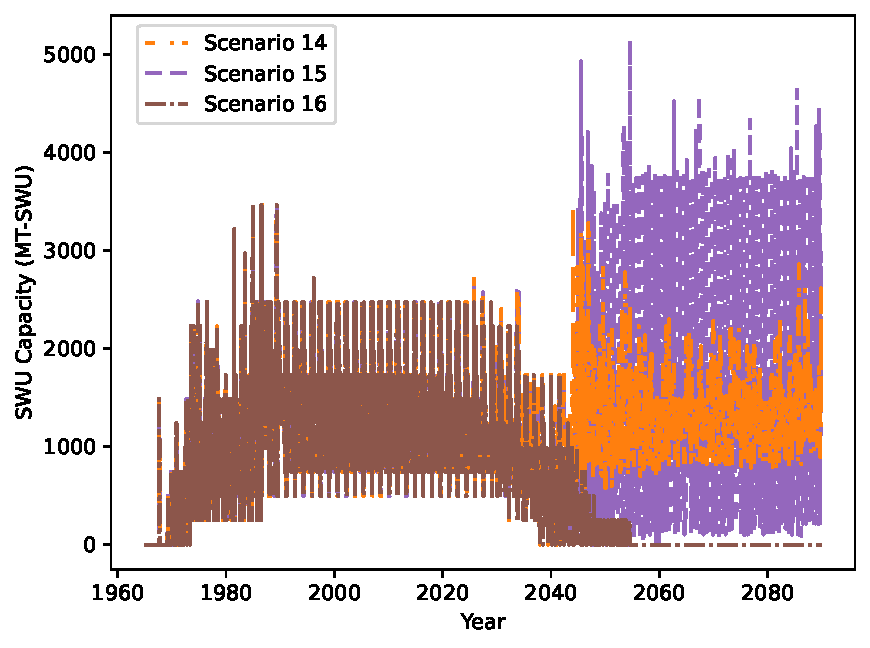
\includegraphics[scale=0.5]{nogrowth_recycle_swu.pdf}
    \end{figure}
\end{frame}

\begin{frame}
    \frametitle{Effects of varying VOYGR build share}
    \begin{figure}
        \centering
        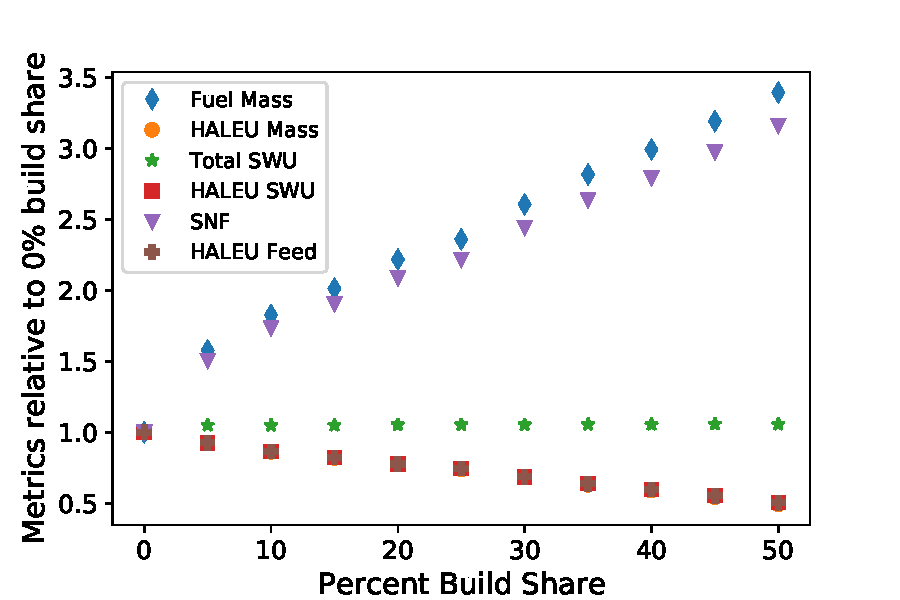
\includegraphics[scale=0.3]{voygr.pdf}
    \end{figure}
\end{frame}

\begin{frame}
    \frametitle{Effects of varying Xe-100 build share}
    \begin{figure}
        \centering
        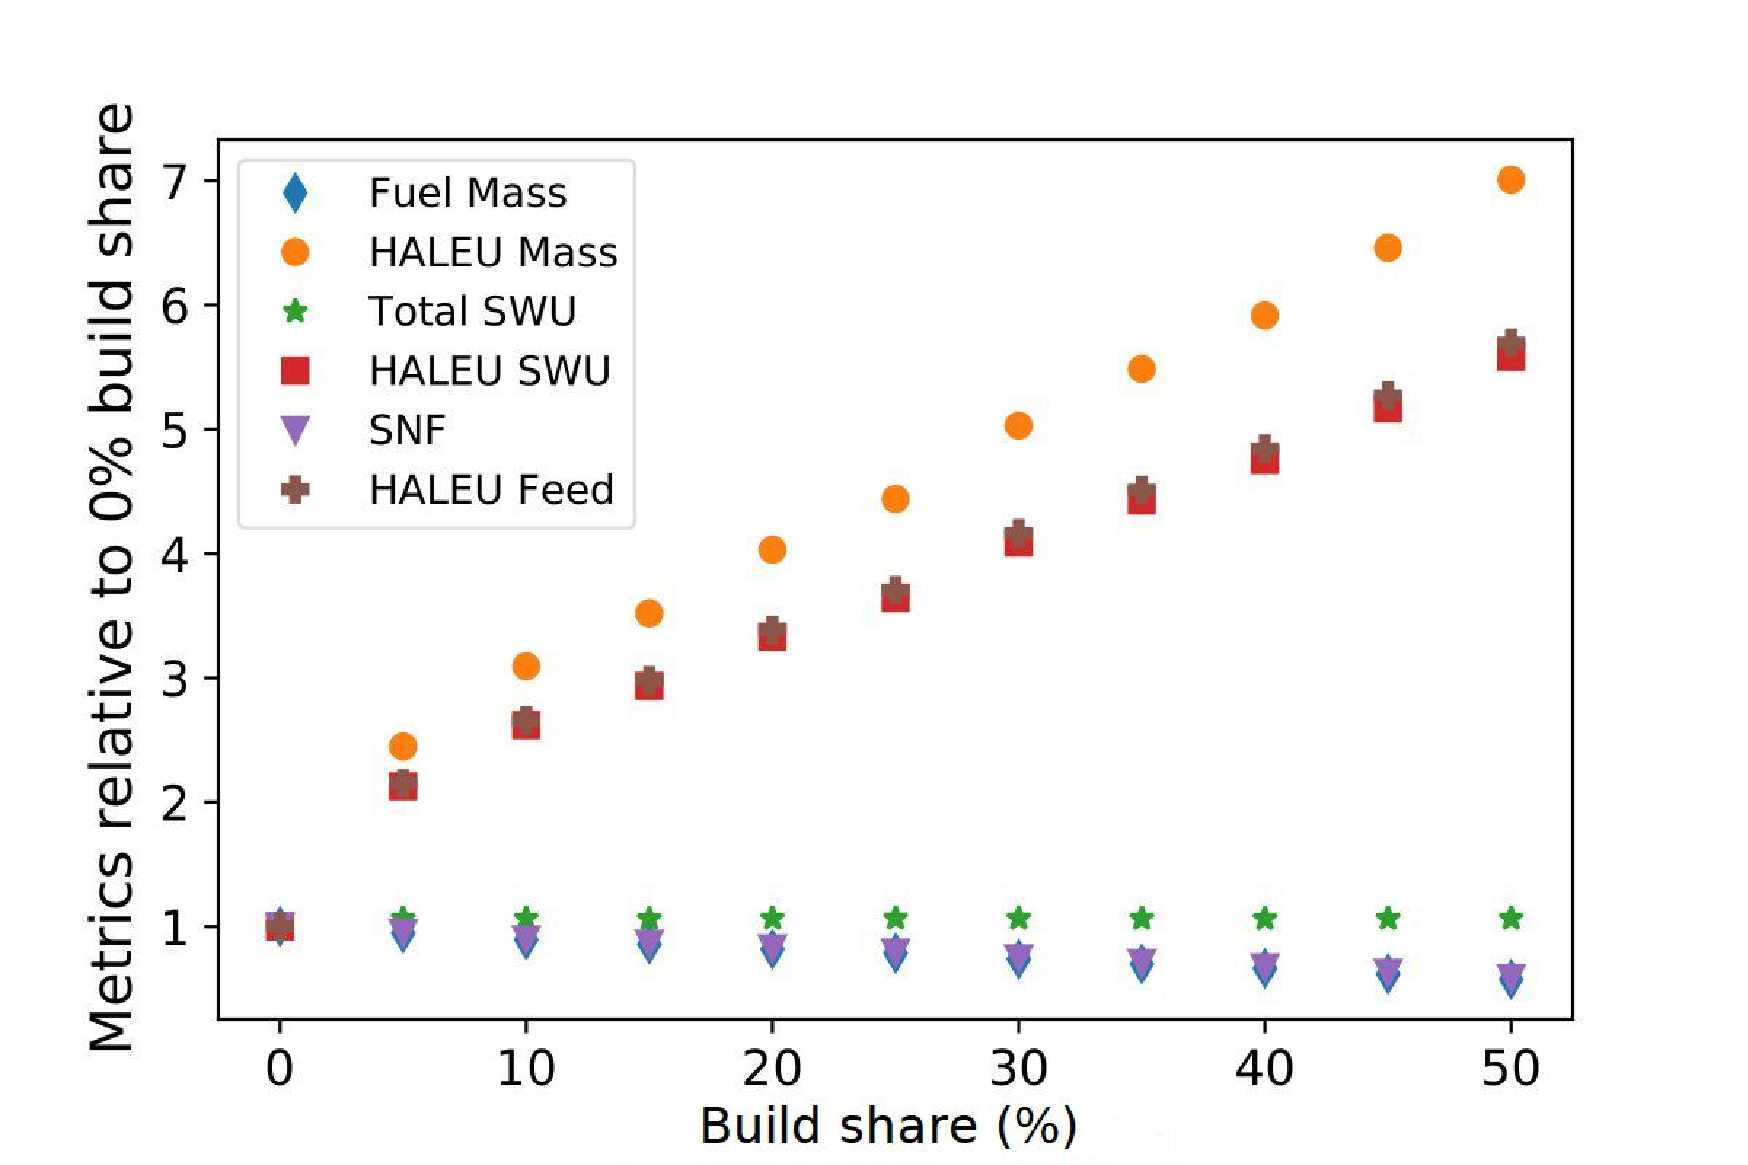
\includegraphics[scale=0.3]{xe100.pdf}
    \end{figure}
\end{frame}
\begin{frame}
    \frametitle{Effects of varying LWR lifetimes}
    \begin{figure}
        \centering
        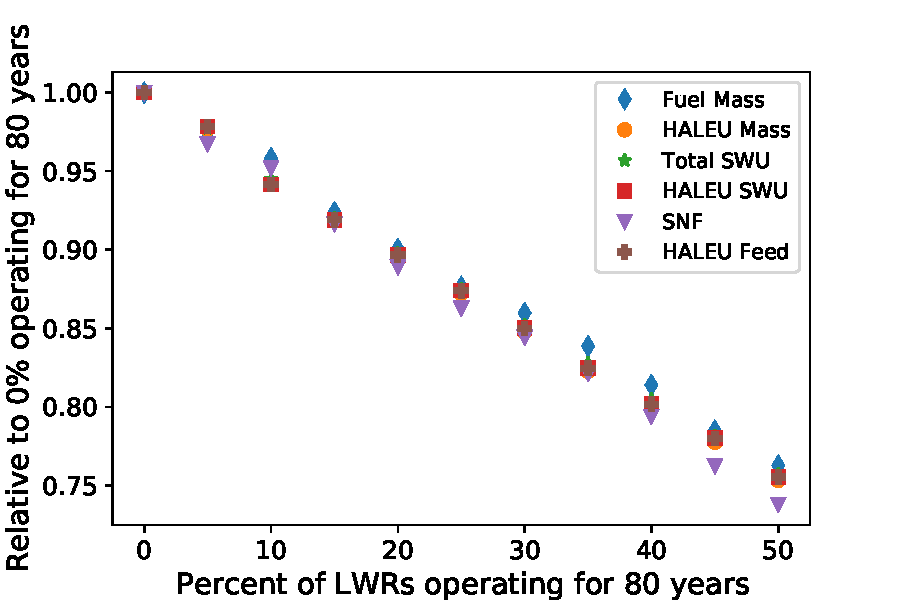
\includegraphics[scale=0.5]{lwr.pdf}
    \end{figure}
\end{frame}
\begin{frame}
    \frametitle{Effects of varying transition start time}
    \begin{figure}
        \centering
        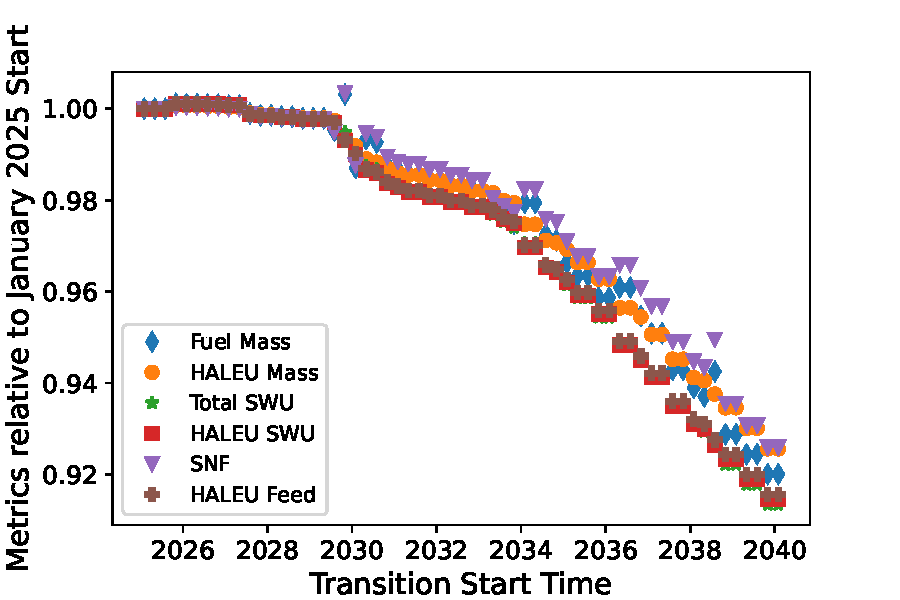
\includegraphics[scale=0.5]{ts.pdf}
    \end{figure}
\end{frame}

\begin{frame}
    \frametitle{HALEU SWU Optimization}
    
\begin{table}[h!]
    \centering 
    \caption{Values resulting in a minimum \gls{HALEU} \gls{SWU} capacity for 
              a once-through transition scenario.}
    \label{tab:soga_ot_haleu}
    \begin{tabular}{c c}
        \hline
        Variable & Value \\
        \hline
        LWR Lifetime & 36\%\\
        Xe-100 build share & 0\%\\
        MMR build share & 2\%\\
        VOYGR build share & 100\%\\
        Xe-100 burnup & 151 MWd/kgU\\
        MMR burnup & 90 MWd/kgU\\
        \hline
        HALEU SWU & 4.812 $\times 10^7$ kg-SWU\\
        \hline
    \end{tabular}
\end{table}
    
\end{frame}

\begin{frame}
    \frametitle{Axial flux through Xe-100}
    \begin{figure}
        \centering 
        \begin{subfigure}{0.49\textwidth}
            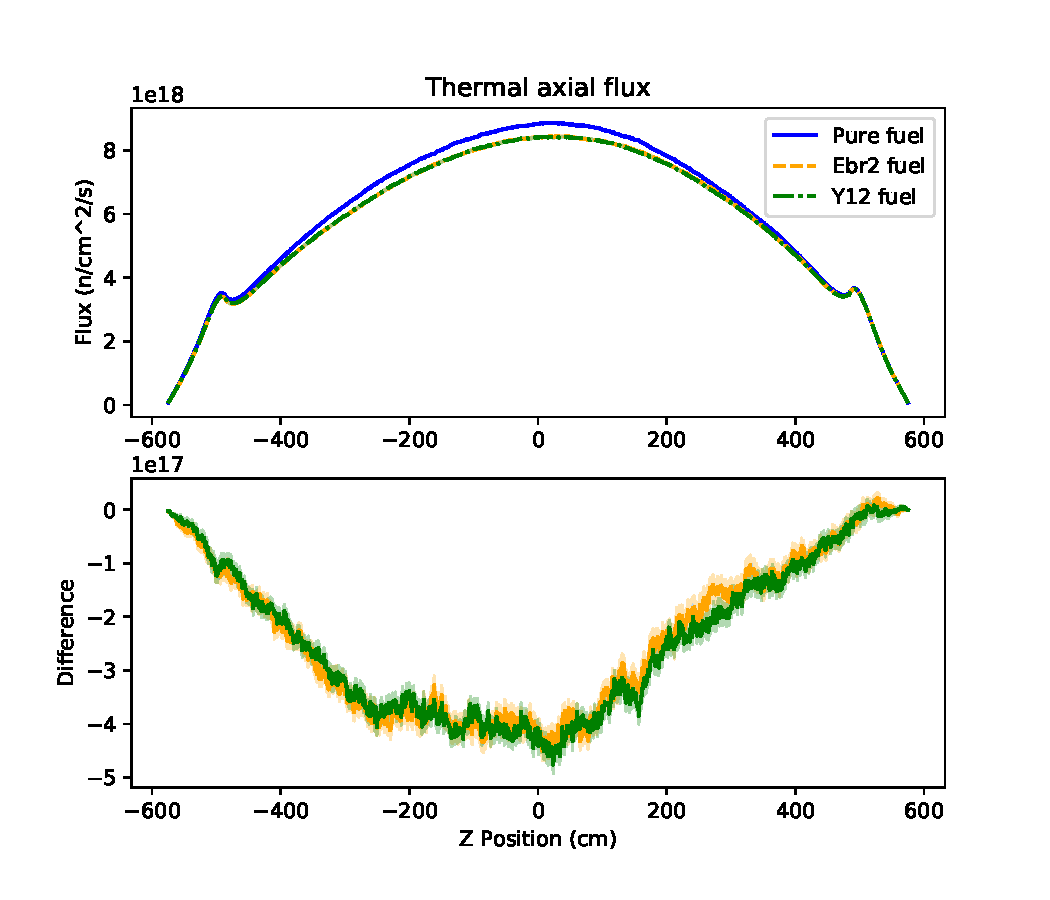
\includegraphics[scale=0.35, trim=20 10 10 20,clip]{xe100_thermal_axial.pdf}
        \end{subfigure}
        \begin{subfigure}{0.49\textwidth}
            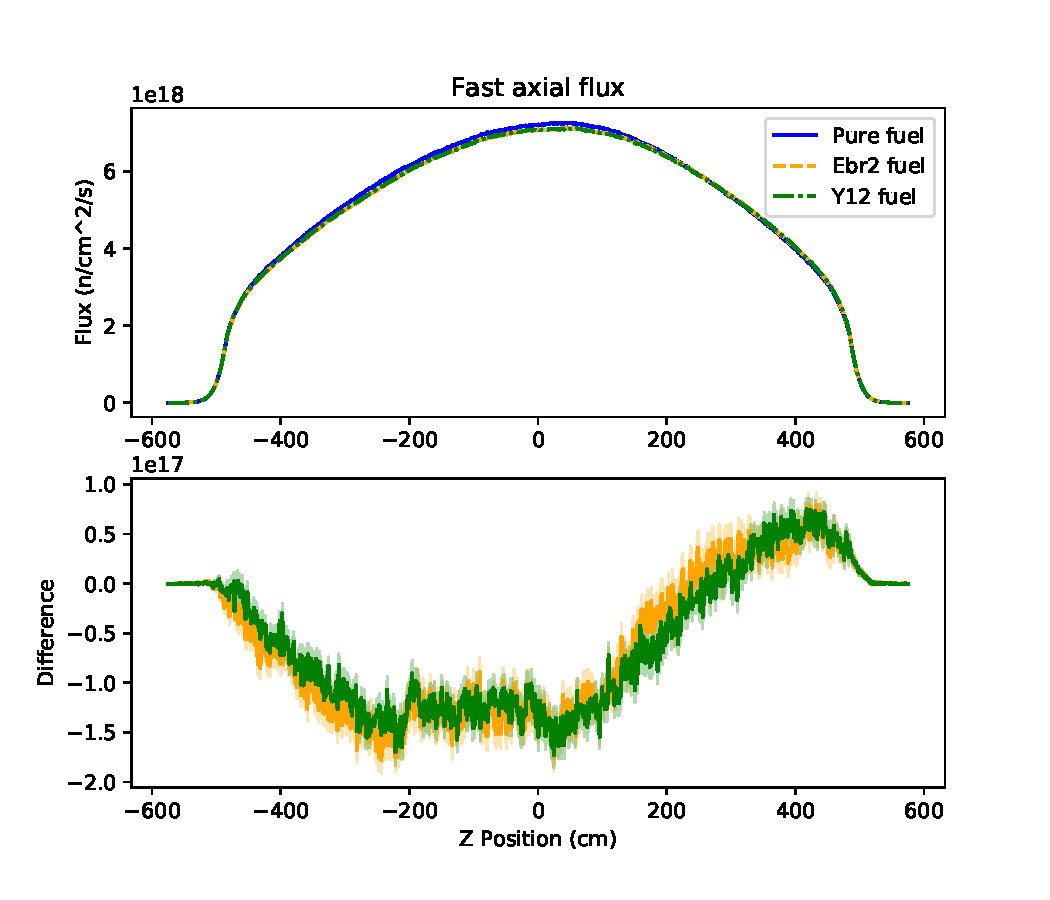
\includegraphics[scale=0.35, trim=10 10 10 20,clip]{xe100_fast_axial.pdf}
        \end{subfigure}
        \caption{Axial fluxes through Xe-100.}
        \label{fig:xe100-axial-flux}
    \end{figure}
\end{frame}

\begin{frame}
    \frametitle{Reactivity feedback coefficients for Xe-100}
    \begin{table}[ht]
        \centering
        \caption{Reactivity temperature feedback coefficients for 
        each material type in the Xe-100-like model for each fuel 
        type.}
        \label{tab:coeff_xe100}
        \begin{tabular}{c c c c c}
            \hline 
            & \multicolumn{4}{c}{Material feedback coefficient (pcm/K)} \\
            Fuel Type & Fuel & Coolant & Moderator & Total \\
            \hline
            Pure & -3.875 $\pm$ 0.094 & -0.044 $\pm$ 0.112 & -0.071 $\pm$ 0.459 & -4.216 $\pm$ 0.502\\
            \gls{EBR} & -3.759 $\pm$ 0.138 & -0.433 $\pm$ 0.048 & -0.708 $\pm$ 0.404 & -4.817 $\pm$ 0.438\\
            Y-12 & -3.797 $\pm$ 0.157 & -0.351 $\pm$ 0.092 & -0.728 $\pm$ 0.469 & -4.700 $\pm$ 0.349\\
            \hline

        \end{tabular}
\end{table}
\end{frame}